\titleframe


%--------------------------------------------------------------------------------



\begin{frame}{Jusqu’à présent, nous avons vu}
    \begin{columns}
  \begin{column}{0.5\textwidth}  
    \begin{itemize}
        \item Ce qu’est un circuit électrique (topologie)
        \item Les grandeurs physiques d’intérêt : courant, tension, puissance, énergie
        \item Les hypothèses faites dans ce cours (circuit localisé, etc.)
        \item Les conventions de sens courant, tension, et les implications sur les puissances consommées, fournies, et leur signe
        \item Les composants R, L, C, transfo, sources indépendantes, sources commandées
    \end{itemize}
  \end{column}
  \begin{column}{0.4\textwidth}
    \begin{itemize}
        \item Les lois de Kirchhoff
        \item Les théorèmes de superposition, de Thévenin et de Norton
        \item L’équivalence de sources
        \item Les régimes transitoires
        \item Le régime sinusoïdal établi, les phaseurs, l’impédance, les puissances actives, réactives, …
        \item Les filtres et AOs
    \end{itemize}
\end{column}
\end{columns}
\end{frame}

\begin{frame}{Vous êtes capables de}
\begin{itemize}
    \item Comprendre le schéma d’un circuit
    \item Calculer les tensions aux n{\oe}uds et courants dans les branches
    \item Réaliser des bilans de puissance
    \item Réduire un circuit complexe en un circuit simple
    \item Optimiser le transfert de puissance d’un circuit vers une charge
    \item Identifier les paramètres d’un modèle d’un circuit sur base de mesures à ses bornes
    \item Déterminer le fonctionnement en régime transitoire
    \item Faire des calculs en RSE avec les phaseurs et impédances
    \item Comprendre ce qu’est un filtre et un amplificateur
\end{itemize}
\end{frame}

\begin{frame}{Qu’allons nous faire dans ce cours ?}
    \begin{itemize}
        \item Systématiser les notions déjà acquises pour \textbf{automatiser} le processus de \textbf{calcul} 
        \item Généraliser le théorème de \textbf{Norton} pour des modèles à\textbf{ plusieurs accès}, utile lorsqu’on souhaite identifier les paramètres ou simplifier un modèle d’une partie d’un circuit “au milieu” d’autres parties
        \item Dans le syllabus : 
        \begin{itemize}
            \item Section 8.1.
            \item Exercices 8.1, 8.4, 8.5, 8.10
        \end{itemize} 
    \end{itemize}
    

\end{frame}

\begin{frame}{Plan du cours}
    \setbeamertemplate{section in toc}[sections numbered]
    \tableofcontents[hideallsubsections]
\end{frame}


\section{La méthode des n{\oe}uds}

\begin{frame}{Introduction et Utilité}
    La mise en équation matricielle permet de :
    \begin{itemize}
        \item \textbf{Systématiser} l'approche d'analyse.
        \item \textbf{Représenter} un circuit via un équivalent Norton multi-accès (ex: quadripôles).
        \item \textbf{Résoudre} numériquement des circuits complexes.
    \end{itemize}
    \vfill
    \begin{block}{Cadre de l'étude}
        Limité ici au \textbf{courant continu (DC)}. Extensible aux phaseurs (AC) et au domaine de Laplace (transitoire).
    \end{block}
\end{frame}

\begin{frame}{Exemple}

    \begin{center}
        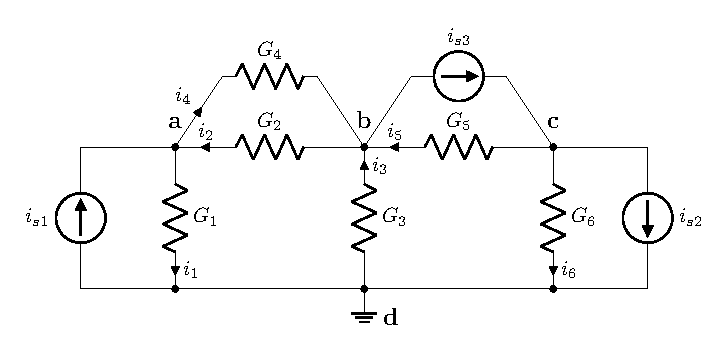
\includegraphics[width=0.7\linewidth]{figs/base_case.pdf}
    \end{center}

    \everycircuitlink{https://everycircuit.com/circuit/6695195064270848}

\end{frame}

\begin{frame}{Vue générale de la méthode}
    Pour déterminer l’état électrique d’un système, la méthode des n{\oe}uds consiste à résoudre le système linéaire suivant :   
    $$\boxed{\mathbf{G}_N \mathbf{v}_N = \mathbf{i}_{sN}}$$
    
    \begin{itemize}
        \item $\mathbf{v}_N$ : Vecteur des \textbf{potentiels de n{\oe}uds} ($n-1$ \alert{variables}).
        \item $\mathbf{G}_N$ : \textbf{Matrice de conductances} aux n{\oe}uds (caractérise le graphe passifié, \alert{paramètres}).
        \item $\mathbf{i}_{sN}$ : Vecteur des \textbf{injections de courant} (sources indépendantes, \alert{paramètres}).
    \end{itemize}
    
    \begin{alertblock}{Condition d'application}
        Circuit linéaire comportant uniquement des sources indépendantes de courant (initialement).
    \end{alertblock}
\end{frame}

\begin{frame}{Algorithme de résolution}    
    \begin{enumerate}
        \item Choisir un \textbf{n{\oe}ud de référence}.
        \item Déterminer la matrice $\mathbf{G}_N$.
        \item Déterminer le vecteur $\mathbf{i}_{sN}$.
        \item Résoudre $\mathbf{G}_N \mathbf{v}_N = \mathbf{i}_{sN}$ pour obtenir les potentiels.
        \item Déduire les courants de branches (Loi d'Ohm).
    \end{enumerate}
\end{frame}

\begin{frame}{Étape 1 : Choisir un n{\oe}ud de référence}
    \begin{itemize}
        \item Généralement choisi comme la masse ou le point commun à toutes les sources.
        \item Tous les potentiels seront exprimés par rapport à ce n{\oe}ud.
        \item Le nombre de variables est réduit à $n-1$, où $n$ est le nombre total de n{\oe}uds.
    \end{itemize}
    \begin{center}
        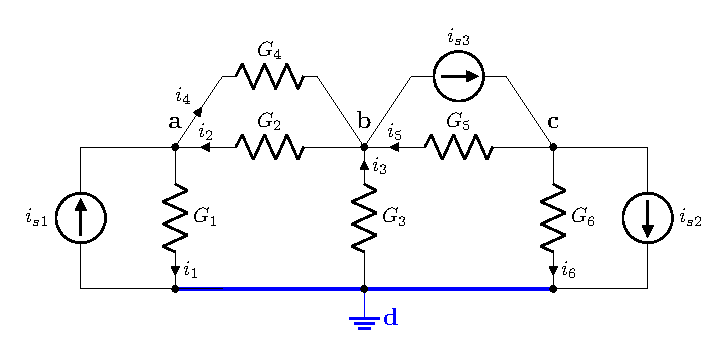
\includegraphics[width=0.7\linewidth]{figs/step_1_reference.pdf}
    \end{center}
\end{frame}

\begin{frame}{Étape 2 : Déterminer la matrice $G_N$}
    \begin{itemize}
        \item $G_N$ est une matrice $(n-1) \times (n-1)$ et caractérise le \alert{circuit passifié}.
    \end{itemize}


\begin{columns}
    \begin{column}{0.7\textwidth}    
        \begin{center}
            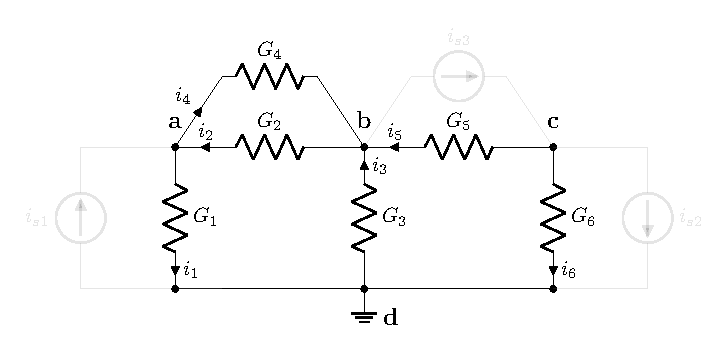
\includegraphics[width=\linewidth]{figs/step_2_passified.pdf}
        \end{center}
    \end{column}
    \begin{column}{0.25\textwidth}
    $\mathrm{G}_{\mathrm{N}}=\left[\begin{array}{lll}? & ? & ? \\ ? & ? & ? \\ ? & ? & ?\end{array}\right]$    
    \end{column}
\end{columns}

\end{frame}

\begin{frame}{Étape 3 : Déterminer le vecteur $i_{sN}$}
    \begin{itemize}
        \item $i_{sN}$ est un vecteur colonne de taille $n-1$.
        \item $\mathrm{i}_{\mathrm{sN}}=\left(\begin{array}{lll}?, & ?, & ? \end{array}\right)$    
    \end{itemize}
        \begin{center}
        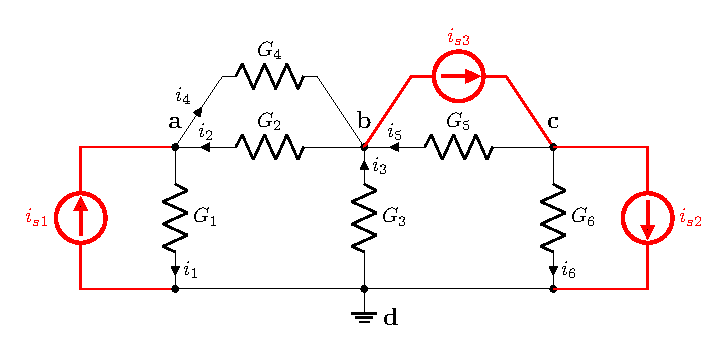
\includegraphics[width=0.6\linewidth]{figs/step_3_current_sources.pdf}
    \end{center}

\end{frame}

\begin{frame}{Étape 4 : Résoudre $G_N v_N = i_{sN}$}
    $\mathrm{v}_{\mathrm{N}}=\left(\begin{array}{lll}?, & ?, & ? \end{array}\right)$    
    \begin{center}
        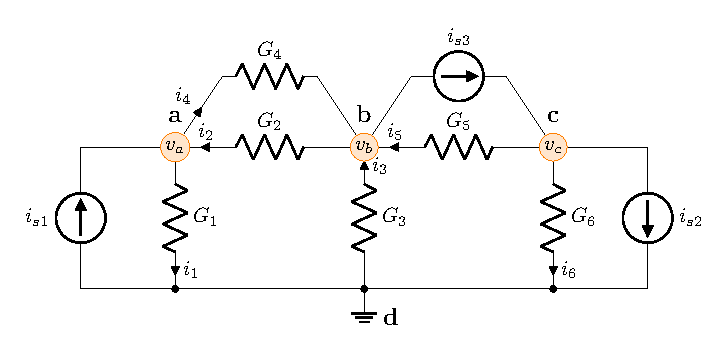
\includegraphics[width=0.6\linewidth]{figs/step4_potentials.pdf}
    \end{center}
\end{frame}


\begin{frame}{Dérivation de la méthode}
    Repose sur trois relations fondamentales :
    \begin{columns}
        \begin{column}{0.5\textwidth}
            \begin{itemize}
                \item \textbf{Loi de Kirchhoff (PLK)} : \\ $\mathbf{A} \mathbf{i}_B = \mathbf{i}_{sN}$
                \item \textbf{Lien Potentiel-Tension} : \\ $\mathbf{u}_B = \mathbf{A}^T \mathbf{v}_{N}$
                \item \textbf{Loi d'Ohm} : \\ $\mathbf{i}_B = \mathbf{G}_B \mathbf{u}_{B}$
            \end{itemize}
        \end{column}
        \begin{column}{0.5\textwidth}
            \begin{block}{Construction de $G_N$}
                En combinant les trois :
                $$\mathbf{A} \mathbf{G}_B (\mathbf{A}^T \mathbf{v}_{N}) = \mathbf{i}_{sN}$$
                D'où la définition :
                $$\mathbf{G}_N \triangleq \mathbf{A} \mathbf{G}_B \mathbf{A}^T$$
            \end{block}
        \end{column}
    \end{columns}

    Où $\mathbf{i}_B$ et $\mathbf{u}_B$ représentent respectivement les vecteurs des courants et tensions de branches (en sens conventionnel).
\end{frame}

\begin{frame}[allowframebreaks]{La Matrice d'Incidence $\mathbf{A}$}

\begin{columns}
  \begin{column}{0.35\textwidth}  
    Elle permet d'écrire sous forme d'expression matricielle les lois de Kirchhoff pour le \textbf{circuit passifié}
    (caractérise donc les relations n{\oe}uds-branches).
  \end{column}
  \begin{column}{0.6\textwidth}
    \begin{center}
        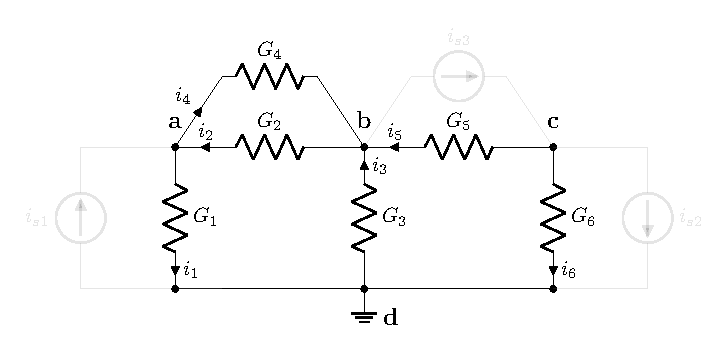
\includegraphics[width=\linewidth]{figs/step_2_passified.pdf}
    \end{center}
  \end{column}
\end{columns}
    
    Ecrivons les relations à tous les n{\oe}uds ($n=4$) : 
    $$\begin{array}{rccccccccccccccccl}
	a & : &  &i_1& -&i_2&  &   & +&i_4&   &     & &   & = & 0\\ 
	b & : &  &   &  &i_2& -&i_3& -&i_4&  -&  i_5& &   & = & 0\\ 
	c & : &  &   &  &   &  &   &  &   &   &  i_5&+&i_6& = & 0\\
	d & : & -&i_1&  &   & +&i_3&  &   &   &     &-&i_6& = & 0
    \end{array}$$

    Si on veut écrire ces relations sous forme matricielle $$A_a \mathbf{i}_b = 0$$ avec $\mathbf{i}_B = (i_1, i_2, i_3, i_4, i_5, i_6)$, alors on peut définir la matrice $A_a$ de dimensions $n \times b$ où chaque élément $a_{ij}$ est défini comme suit:
\begin{enumerate}
\item $a_{ij} = -1$ si la branche $j$ est incidente au n{\oe}ud $i$ et est orientée vers lui ;
\item $a_{ij} = +1$ si la branche $j$ est incidente au n{\oe}ud $i$ et est orientée en sens opposé ;
\item $a_{ij} = 0$ si la branche $j$ n'est pas incidente au n{\oe}ud $i$
\end{enumerate}
Ici, on a donc 
    $$A_a = \left[\begin{array}{rrrrrr}
	   1& -1&  0&  1&   0& 0 \\ 
	   0&  1& -1& -1&  -1& 0 \\ 
	   0&  0&  0&  0&   1& 1 \\
	  -1&  0&  1&  0&   0&-1
    \end{array} \right]$$

    Cette matrice est cependant de rang $n-1$, car une PLK peut-être déduite des $n-1$ autres. 
    Par exemple ici, la PLK au n{\oe}ud $d$ s'obtient à partir des trois premières relations.

    On définit la matrice d'incidence réduite $A$ en conservant $n-1$ relations linéairement indépendantes, correspondant à tous les n{\oe}uds sauf celui de référence (ici $d$):
    $$\mathbf{A} = \left[\begin{array}{rrrrrr}
	   1& -1&  0&  1&   0& 0 \\ 
	   0&  1& -1& -1&  -1& 0 \\ 
	   0&  0&  0&  0&   1& 1
    \end{array} \right]$$
\end{frame}

\begin{frame}{Déterminer le vecteur ${\bf i}_{sN}$}

\begin{columns}
  \begin{column}{0.35\textwidth}
Si on considère maintenant le circuit complet,

    $$\begin{array}{rrl}
a: & i_1-i_2+i_4& =i_{s 1} \\
b: & i_2-i_3-i_4-i_5& =-i_{s 3} \\
c: & i_5+i_6& =i_{s 3}-i_{s 2}
\end{array}$$
  \end{column}
  \begin{column}{0.6\textwidth}
    \begin{center}
        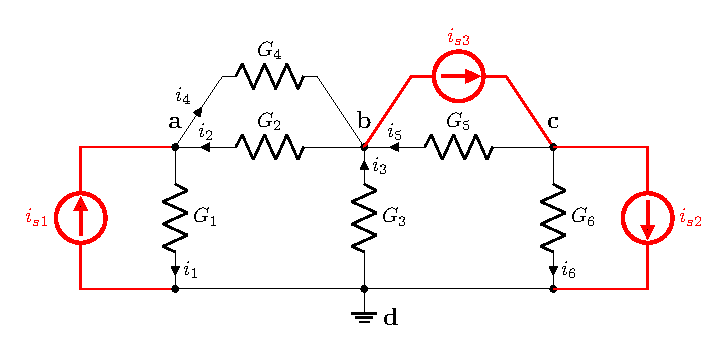
\includegraphics[width=\linewidth]{figs/step_3_current_sources.pdf}
    \end{center}  
  \end{column}
\end{columns}
\begin{columns}
  \begin{column}{0.45\textwidth}
    par comparaison avec la relation 
$$\mathbf{A} \mathbf{i}_B = \mathbf{i}_{sN}$$

\end{column}
  \begin{column}{0.45\textwidth}    
    On a 
    \[ {\bf i}_{sN} = 
    \left[
        \begin{array}{c}
            i_{s1}\\
            -i_{s3}\\
            i_{s3}-i_{s2}
        \end{array} \right] \]
    \end{column}
    \end{columns}
\end{frame}

\begin{frame} {Lien entre potentiel et tension de branche}

    La matrice $\mathbf{A}$ encode la topologie du réseau. Elle permet donc aussi de relier les tensions de branche aux potentiels :
    $$\mathbf{u}_B = \mathbf{A}^T \mathbf{v}_{N}.$$
Pour notre exemple :

\begin{columns}
  \begin{column}{0.55\textwidth}
  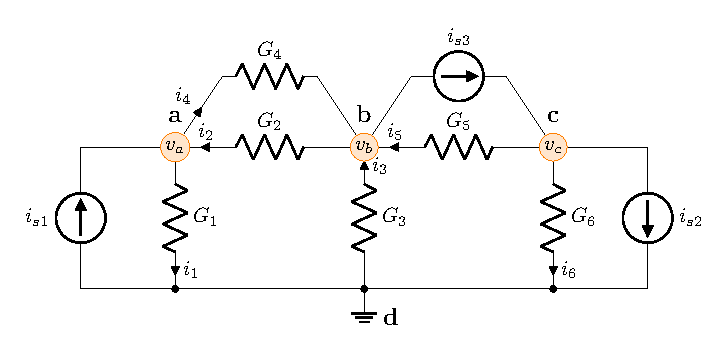
\includegraphics[width=\textwidth]{figs/step4_potentials.pdf}
  \end{column}
  \begin{column}{0.35\textwidth}
    $$
    \left[\begin{array}{l}
        u_1 \\
        u_2 \\
        u_3 \\
        u_4 \\
        u_5 \\
        u_6 
    \end{array}\right]=\left[\begin{array}{rrr}
        1 & 0 & 0 \\
        -1 & 1 & 0 \\
        0 & -1 & 0 \\
        1 & -1 & 0 \\
        0 & -1 & 1 \\
        0 & 0 & 1
    \end{array}\right]\left[\begin{array}{l}
        v_a \\
        v_b \\
        v_c
    \end{array}\right]
    $$
\end{column}
\end{columns}
\end{frame}

\begin{frame}{La dernière étape : la loi d'Ohm}
    Elle permet de relier courants et tensions de branche. Sous forme matricielle, elle se traduit par
    $$\mathbf{i}_B = \mathbf{G}_B \mathbf{u}_{B}.$$
    Avec ${\bf G}_B$ la matrice diagonale
    \[{\bf G}_B = \left[
\begin{array}{cccc}
G_1 & \\
& G_2 & {\bf 0} & \\
&  {\bf 0} & \ddots \\
& & & G_b
\end{array} \right]\]
\end{frame}

\begin{frame}{Application de la méthode des n{\oe}uds}
    Une fois le n{\oe}ud de référence choisi, la méthode se résume donc à :
    \begin{enumerate}
        \item construire $\mathbf{A}$
        \item construire $\mathbf{G}_B$
        \item en déduire $\mathbf{G}_N \triangleq \mathbf{A} \mathbf{G}_B \mathbf{A}^T$
        \item construire $\mathbf{i}_{sN}$
        \item résoudre $\mathbf{G}_N \mathbf{v}_N = \mathbf{i}_{sN}$
    \end{enumerate} 

    Il est possible de simplifier les étapes 1 à 3 grâce à la \textbf{méthode d'inspection}...

\end{frame}

\begin{frame}{Détermination de $\mathbf{G}_N$ par inspection}

\begin{columns}
  \begin{column}{0.3\textwidth}
    Si $\mathbf{G}_B$ est diagonale (pas de sources commandées), alors on peut déterminer les éléments de $\mathbf{G}_N$ par inspection :
  \end{column}
  \begin{column}{0.65\textwidth}
    \begin{table}
        \centering
        \begin{tabular}{l p{4cm}}
            \hline
            \textbf{Terme} & \textbf{Règle} \\ \hline
            $G_{ii}$ (Diagonal) & Somme des conductances incidentes au n{\oe}ud $i$. \\
            $G_{ik}$ (Hors-diag) & \textbf{Opposé} de la somme des conductances liant les n{\oe}uds $i$ et $k$. \\ \hline
        \end{tabular}
    \end{table}
\end{column}
\end{columns}
\begin{columns}
  \begin{column}{0.55\textwidth}
  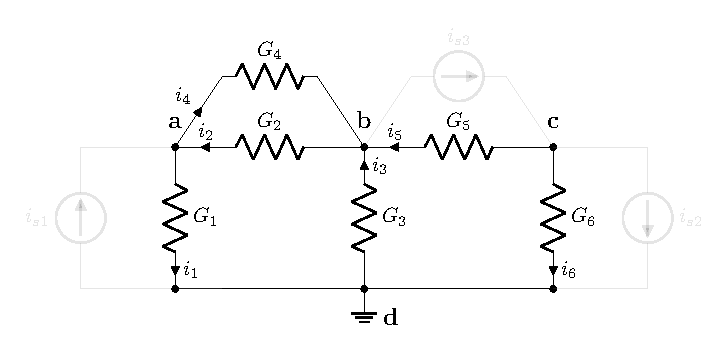
\includegraphics[width=\textwidth]{figs/step_2_passified.pdf}
  \end{column}
  \begin{column}{0.35\textwidth}
        $G_{11} = G_1 + G_2 + G_4$ \\
        $G_{12} = -(G_2 + G_4)$\\
        ...
\end{column}
\end{columns}
\end{frame}




\begin{frame}{Détermination de $\mathbf{G}_N$ par inspection}
Pour l'exemple précédent, on a directement 
\[
{\bf G}_N =
\left[ \begin{array}{ccc}
G_1+G_2+G_4 & -(G_2+G_4) & 0 \\
-(G_2+G_4) & G_2+G_3+G_4+G_5 & -G_5\\
0 & -G_5 & G_5+G_6
\end{array} \right]. \]

\vspace{1cm}

\textit{Pourquoi ?} La matrice $\mathbf{A} \mathbf{G}_B \mathbf{A}^T$ est la\textbf{ matrice Laplacienne pondérée du graphe}.
On peut établir ces formules en développant le produit matriciel et en tenant compte du fait que chaque colonne de $\mathbf{A}$, qui représent une arrête du graphe, comporte maximum 2 éléments non-nuls valant $1$ ou $-1$.

\end{frame}

\begin{frame}{Revenons à notre exemple}

Données : $i_{s1} = 3$ mA, $i_{s2} = 1$ mA, $i_{s3} = 5$ mA, et toutes les résistances valent $1$ $k\Omega$ (donc $1$ mS).
Par inspection, 
$$
{\bf G}_N = 10^{-3}
\left[ \begin{array}{ccc}
3 & -2 & 0 \\
-2 & 4 & -1\\
0 & -1 & 2
\end{array} \right] \text{ S}$$
et 
$$\mathbf{i}_{sN} = 10^{-3}(3, -5, 4) \text{ A}$$
On obtient (avec la calculatrice Numworks, encoder les matrices via la touche "Toolbox/Matrice et vecteurs")
$$\mathbf{v}_{N} = {\bf G}_N^{-1}\mathbf{i}_{sN} =  \frac{1}{13}(9, -6, 23) \text{ V}$$

\everycircuitlink{https://everycircuit.com/circuit/6695195064270848}


\end{frame}

\begin{frame}[allowframebreaks]{Réseau équivalent}
    
    \begin{columns}
      \begin{column}{0.4\textwidth}
Lorsque le circuit est mis en équation grâce à la méthode des n{\oe}uds, il peut être remplacé par un circuit équivalent constitué du
circuit passifié vu de $n-1$ accès auxquels agissent des sources indépendantes de courant équivalentes regroupant les sources indépendantes du circuit original.
\end{column}
\begin{column}{0.5\textwidth}
    \begin{center}
        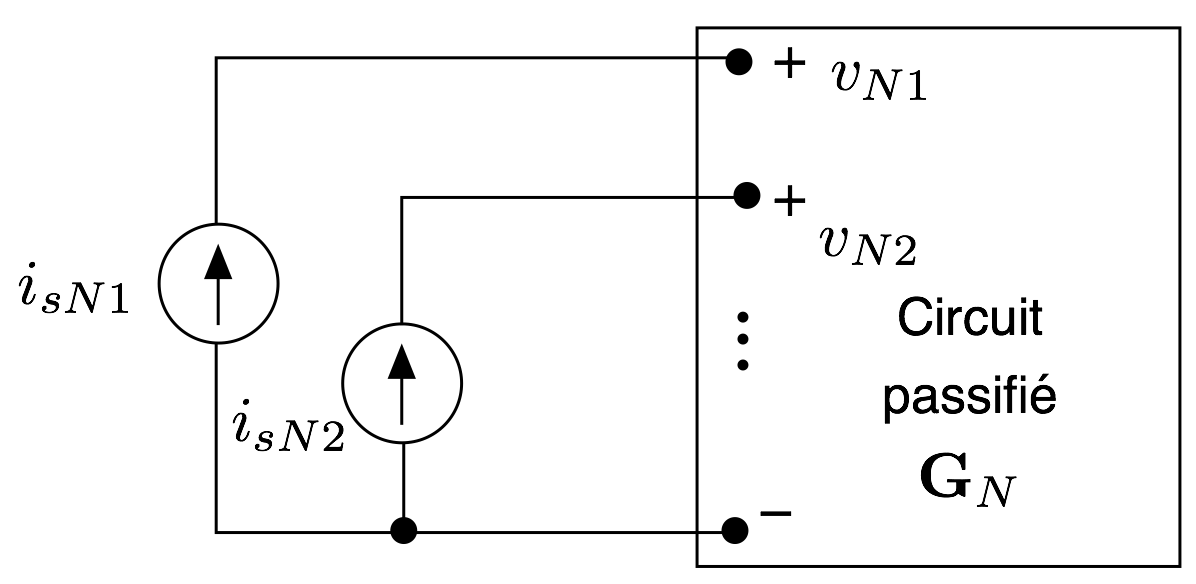
\includegraphics[width=\linewidth]{figs/reseau_equivalent_MN}
    \end{center}
\end{column}
\end{columns}

\begin{center}
    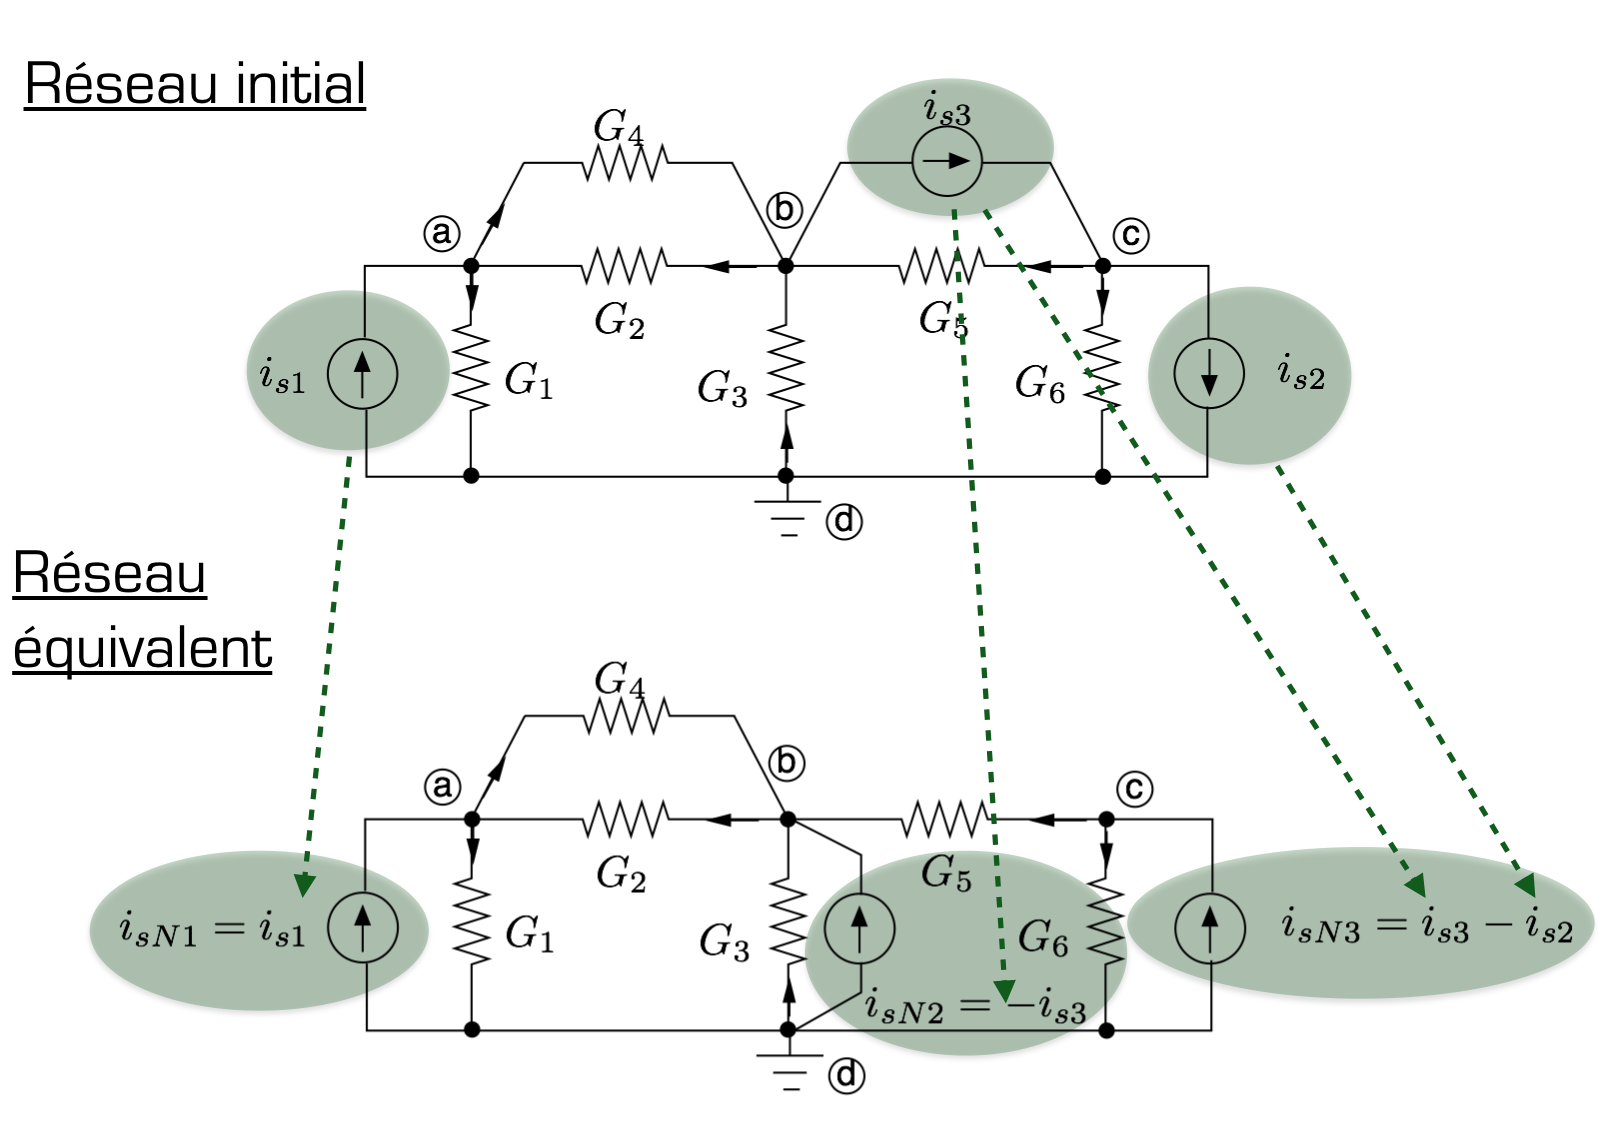
\includegraphics[width=0.7\linewidth]{figs/ex_reseau_equivalent_MN}
\end{center}
\end{frame}

\section{Cas particuliers et méthode d'expérimentation}
\begin{frame}{Cas particuliers : Sources de tension}
    Comment gérer une source de tension indépendante ?
    \begin{itemize}
        \item \textbf{En série avec R} : Transformation de Thévenin vers Norton (Source de courant en parallèle).
        \item \textbf{Source de tension seule} : Transformation du circuit pour "pousser" la source à travers les n{\oe}uds adjacents.
    \end{itemize}
    \begin{center}
        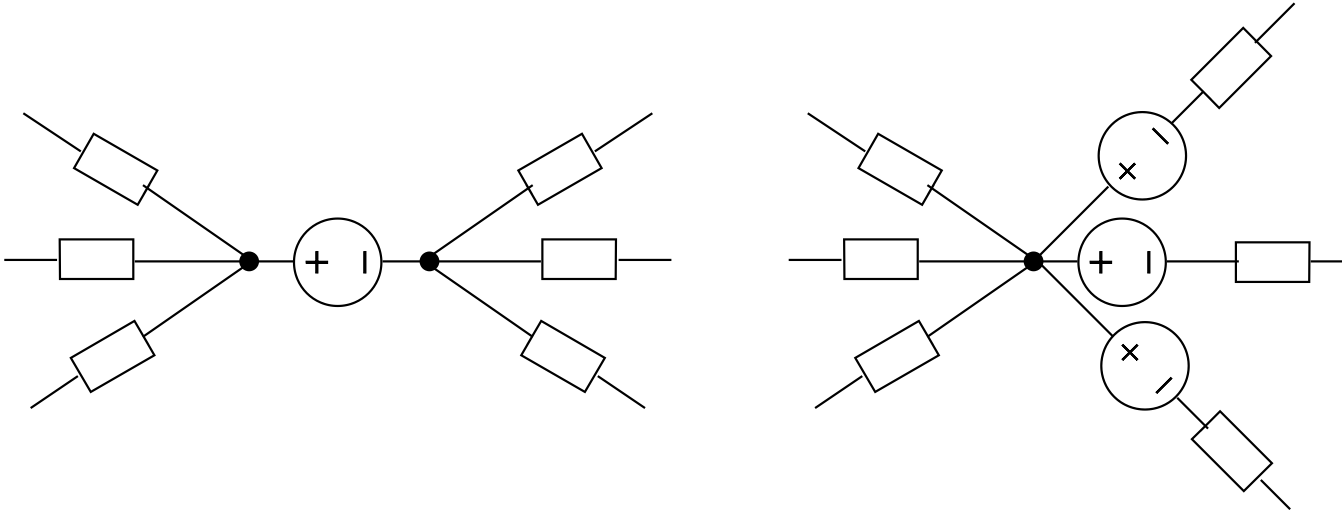
\includegraphics[width=0.7\linewidth]{figs/transformation_SIV}
    \end{center}
\end{frame}

\begin{frame}[allowframebreaks]{Cas particuliers : Sources commandées (VCT)}

\begin{columns}
  \begin{column}{0.6\textwidth}
    \begin{center}
        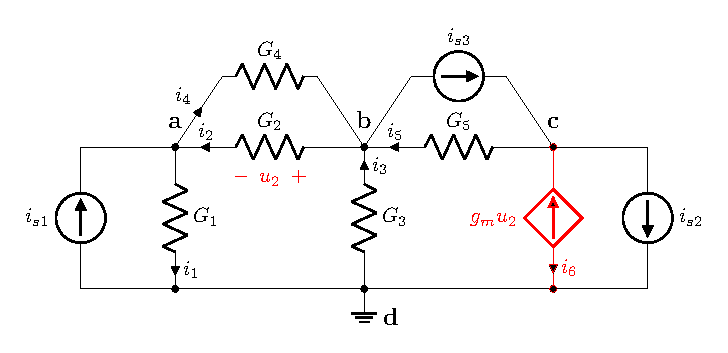
\includegraphics[width=\linewidth]{figs/base_case_with_VCT.pdf}
    \end{center}
  \end{column}
  \begin{column}{0.35\textwidth}
    Pour une source de courant commandée par une tension ($i = g_m u$) :
    \begin{itemize}
        \item La matrice $\mathbf{G}_B$ n'est plus diagonale.
        \item La matrice $\mathbf{G}_N = \mathbf{A} \mathbf{G}_B \mathbf{A}^T$ devient \textbf{asymétrique}.
        \item L'inspection directe devient difficile ; privilégier 
        \begin{itemize}
            \item le calcul matriciel 
            \item l'\textbf{expérimentation}.
        \end{itemize} 
    \end{itemize}
  \end{column}
\end{columns}

\newpage
Dans notre exemple, 
  \begin{itemize}
    \item la matrice d'incidence est inchangée car la topologie est inchangée, 
    \item mais le courant $i_6 = -g_m u_2$ dépend de la tension de la branche 2, donc 
     \[{\bf G}_B=
\left[
\begin{array}{cccccc}
G_1 & 0 & 0 & 0 & 0 & 0\\
0 & G_2 & 0 & 0 & 0 & 0 \\
0 & 0 & G_3 & 0 & 0 & 0\\
0 & 0 & 0 & G_4 & 0 & 0\\
0 & 0 & 0 & 0 & G_5 & 0\\
0 & \mathcolor{red}{-g_m}& 0 & 0 & 0 & \mathbf{0}
\end{array}\right]\]
  \end{itemize}
  
Dès lors, 
\[{\bf G}_N={\bf A}{\bf G}_B{\bf A}^T= 
\left[
\begin{array}{ccc}
G_1+G_2+G_4 & -(G_2+G_4) & \mathbf{0} \\
-(G_2+G_4) & G_2+G_3+G_4+G_5 & \mathbf{-G_5} \\
\mathcolor{red}{g_m} & -(G_5\mathcolor{red}{+g_m}) & G_5
\end{array}\right]\]
\end{frame}

\begin{frame}[allowframebreaks]{Méthode d'expérimentation}

    On utilise la méthode d'expérimentation lorsque 
    \begin{itemize}
        \item le circuit comporte des couplages entre branches
        \item on n'a pas accès aux paramètres du circuit mais on peut prendre des mesures
    \end{itemize}
    

    Elle exploite la représentation du circuit par un réseau équivalent. 
    En effet, ${\bf G}_N$ caractérise le circuit passifié. Les relations $i-u$ aux $n-1$ accès s'écrivent : 
\begin{eqnarray*}
	i_{1} & = & G_{11}v_{1} + G_{12}v_{2}+ \ldots \\
	i_{2} & = & G_{21}v_{1} + G_{22}v_{2}+ \ldots 
\end{eqnarray*}
où ${\bf i}$ est le vecteur des courants injectés aux accès, ${\bf v}$ est le vecteur des tensions aux accès.

\begin{block}{Règle d'expérimentation pour déterminer les éléments de $\mathbf{G}_N$}
\[G_{ij}= i_{i}|_{v_{j}=1, v_{k}=0,k\neq j}\]
\begin{itemize}
	\item Imposer une tension de $1 V$ à l'accès $j$
	\item Court-circuiter les autres accès
	\item Déterminer dans ces conditions le courant à l'accès $i$
\end{itemize}
\end{block}

\newpage

Les éléments de ${\bf G}_N$ sont alors déterminés par des essais successifs, illustrés ci-dessous :
\begin{columns}
  \begin{column}{0.45\textwidth}
    \begin{center}        
      Sur la diagonale \\
      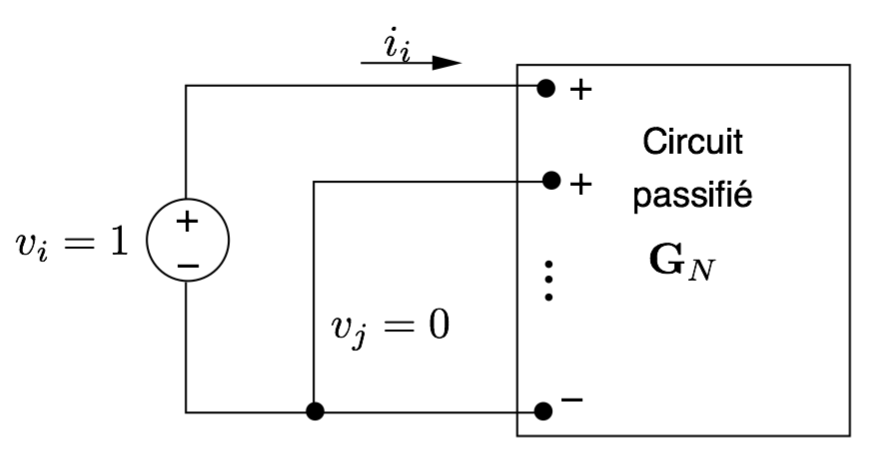
\includegraphics[width=\linewidth]{figs/experimentation_ii.png}
    \end{center}
  \end{column}
  \begin{column}{0.45\textwidth}
    \begin{center}
        Hors diagonale\\
        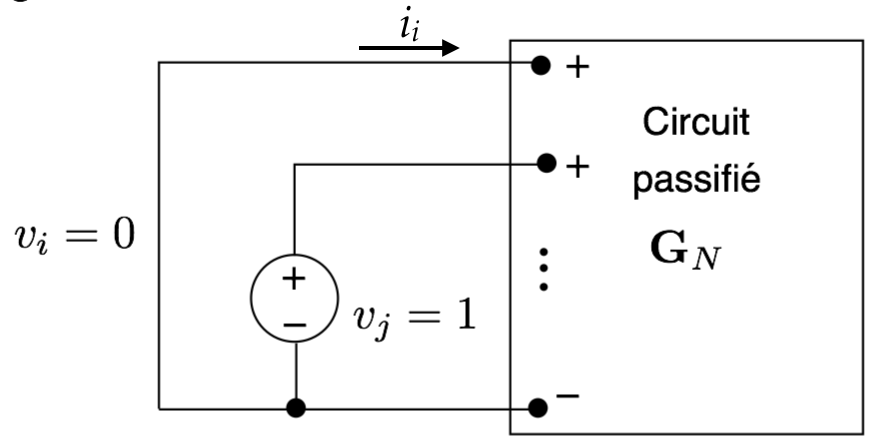
\includegraphics[width=\linewidth]{figs/experimentation_ij.png}        
    \end{center}
  \end{column}
\end{columns}

\end{frame}

\begin{frame}[allowframebreaks]{Exemple d'application de la méthode d'expérimentation}
Reprenons l'exemple précédent contenant une source VCT.
Calculons quelques éléments de ${\bf G}_N$. Commençons par 
\[G_{31}=i_{3}|_{v_{1}=1,v_{2}=v_{3}=0}\]
ce qui se traduit par l'expérience suivante : 

\begin{columns}
  \begin{column}{0.5\textwidth}
    \begin{center}
    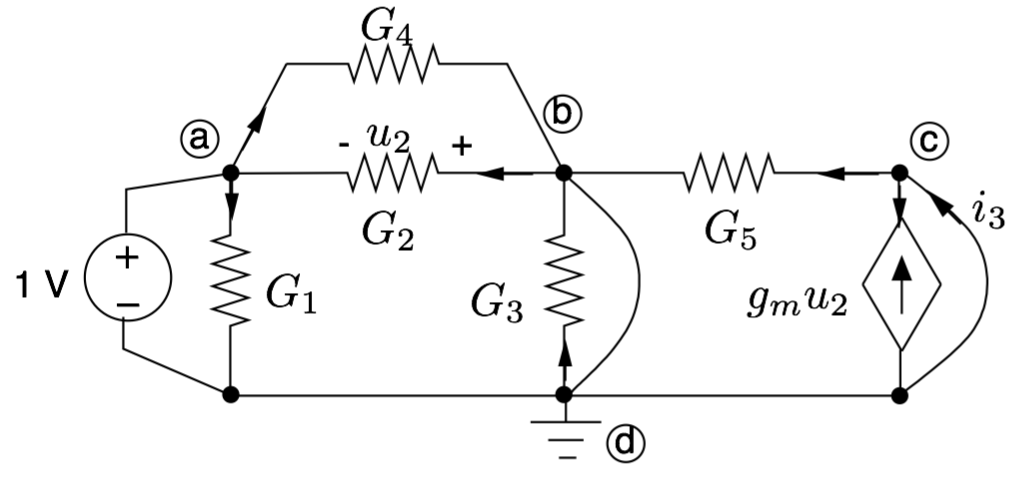
\includegraphics[width=\linewidth]{figs/ex_exp_1}
    \end{center}  
  \end{column}
  \begin{column}{0.35\textwidth}
On a successivement 
\begin{align*}
u_5&=0 \\
i_5&=0 \\
u_2&=-1 \\
i_6&=-g_mu_2=g_m \\
G_{31} &= i_{3}= i_5+i_6=g_m
\end{align*}
  \end{column}
\end{columns}

De même pour \[G_{32}=i_{3}|_{v_{2}=1,v_{1}=v_{3}=0}\]

\begin{columns}
  \begin{column}{0.55\textwidth}
    \begin{center}
        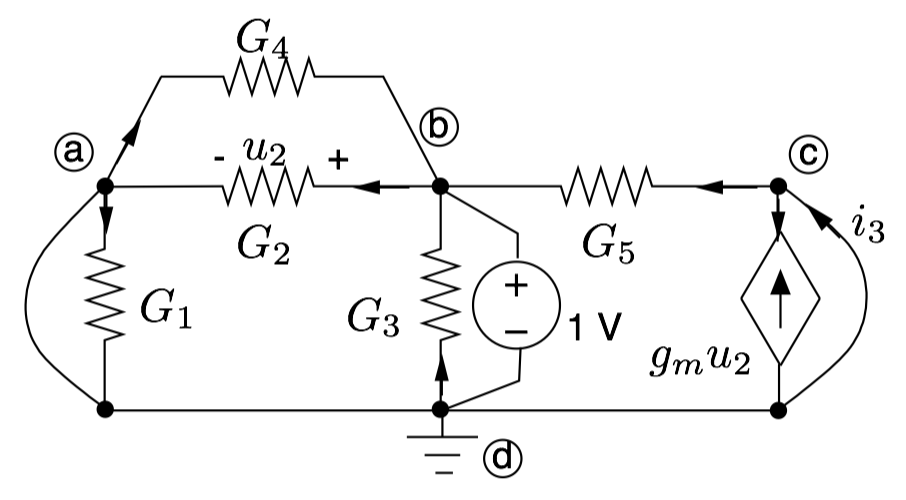
\includegraphics[width=\linewidth]{figs/ex_exp_2}
    \end{center}
  \end{column}
  \begin{column}{0.35\textwidth}
    on a 
    \begin{align*}
    u_5&=-1 \\
    i_5&=-G_5 \\
    u_2&=1 \\
    i_6&=-g_mu_2=-g_m\\
    G_{32} & =  i_{3}= i_5+i_6 =  -(G_5+g_m)
    \end{align*}
  \end{column}
\end{columns}
Finalement, pour \[G_{33}=i_{3}|_{v_{3}=1,v_{1}=v_{2}=0}\]

\begin{columns}
  \begin{column}{0.55\textwidth}
    \begin{center}
        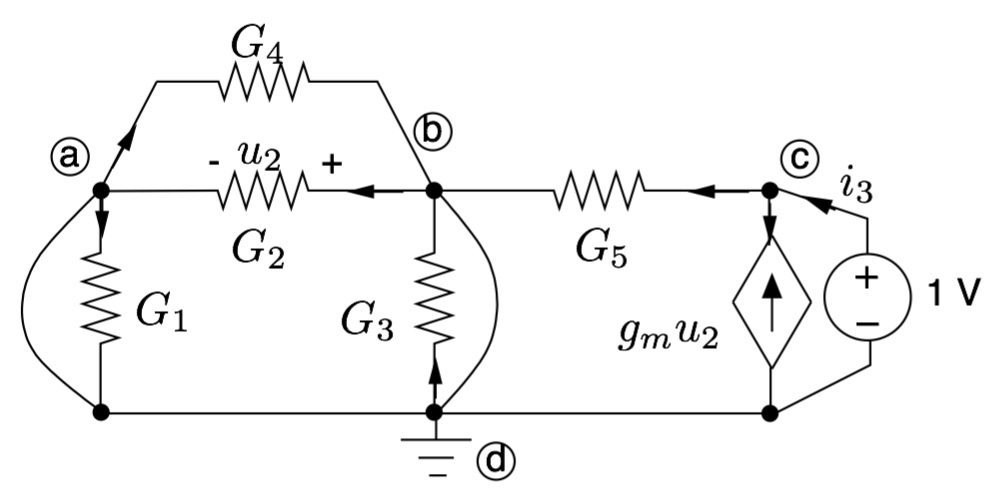
\includegraphics[width=\linewidth]{figs/ex_exp_3}
    \end{center}  
  \end{column}
  \begin{column}{0.35\textwidth}
    on a
    \begin{align*}
    u_5&=1 \\
    i_5&=G_5 \\
    u_2&=0 \\
    i_6&=0 \\
    G_{33} &= i_{3}= i_5+i_6=G_5.
    \end{align*}
  \end{column}
\end{columns}

\newpage 

Remarques:
\begin{itemize}
    \item $n-1$ expériences suffisent (dans ce cas 3) pour déterminer tous les éléments. En effet dans chaque expérience, on aurait pu déterminer les $n-2$ autres courants (ici $i_1$ et $i_2$) et donc compléter la matrice.
    \item la source de courant commandée injecte au n{\oe}ud $c$ en fonction de la différence de potentiel entre les n{\oe}uds $b$ et $a$. Ce sont donc les éléments $(3,1)$ et $(3,2)$ qui sont impactés par $g_m$.
\end{itemize}


\end{frame}

\section{Equivalent de Norton à plusieurs accès}

\begin{frame}{Motivation}
    \begin{center}
    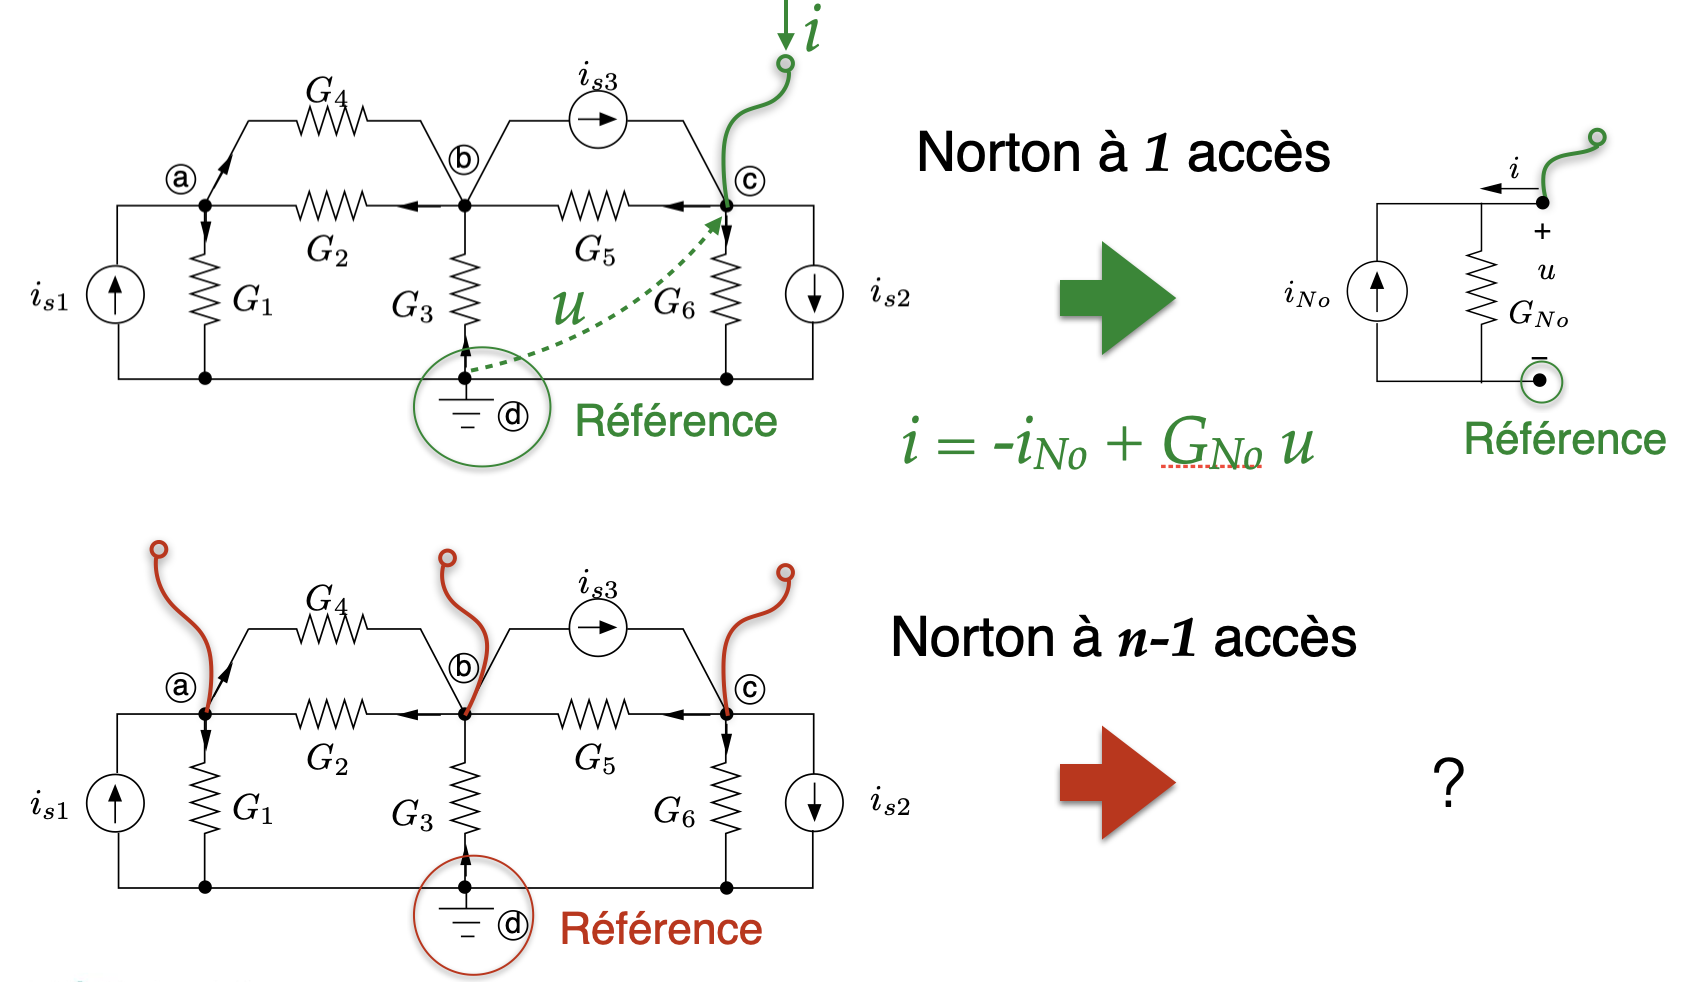
\includegraphics[width=0.8\linewidth]{figs/illu_Norton.png}    
    \end{center}
\end{frame}

\begin{frame}{Généralisation du Théorème de Norton à plusieurs accès}

    Considérons le schéma équivalent du circuit déduit de la méthode des n{\oe}uds, avec $N=n-1$ accès ; un accès entre chaque n{\oe}ud et le n{\oe}ud de référence, aux bornes de chaque source équivalente de courant.


\begin{columns}
    \begin{column}{0.45\textwidth}
      \begin{center}
      
\includegraphics[width=\linewidth]{figs/norton}
      \end{center}
    \end{column}
  \begin{column}{0.45\textwidth}
    Les relations $i-u$ pour les $N$ accès sont
    \[{\bf i}=-{\bf i}_{sN}+{\bf G}_N{\bf v}_N\]
    ou encore
    \[{\bf i}=-{\bf i}_{sN}+{\bf G}_N{\bf u}\]
    On en déduit le schéma équivalent de Norton à $N$ accès par simple identification :
    \[ {\bf i}_{No} = {\bf i}_{sN}\,\, , \quad \quad {\bf G}_{No}={\bf G}_{N}\]  
  \end{column}
\end{columns}

\end{frame}

\begin{frame}[allowframebreaks]{Réduction du nombre d'accès}

    \begin{columns}
        \begin{column}{0.45\textwidth}
            Considérons maintenant que parmis les $N$ accès, un sous-enesemple d'accès $a$ est jugé intéressant, alors que les $b$ autres accès sont laissés "ouverts" ($\mathbf{i}_b = 0$).
        \end{column}
        \begin{column}{0.45\textwidth}
          \begin{center}
          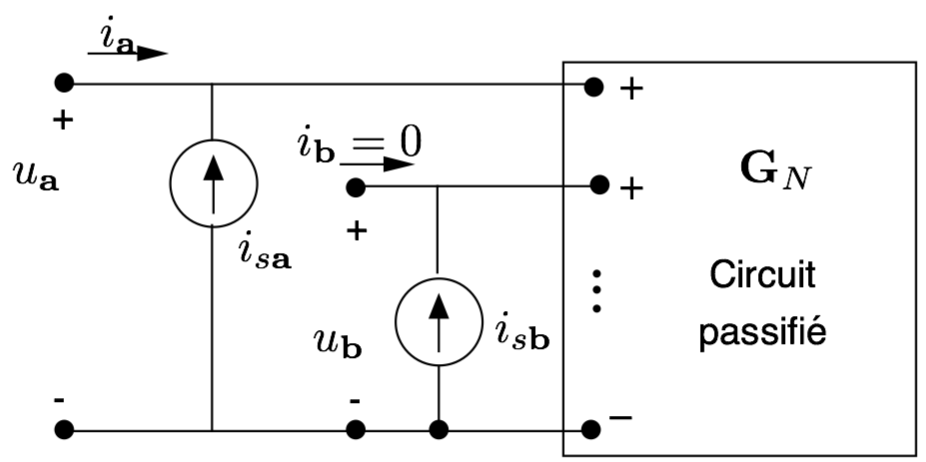
\includegraphics[width=\linewidth]{figs/reduction.png}
          \end{center}
        \end{column}
\end{columns}

    Pour obtenir un équivalent de Norton \alert{sur $a$ accès parmi $N$}, partitionons les matrices :
    $$ \begin{bmatrix} \mathbf{i}_a \\ \mathbf{i}_b \end{bmatrix} = - \begin{bmatrix} \mathbf{i}_{sa} \\ \mathbf{i}_{sb} \end{bmatrix} + \begin{bmatrix} \mathbf{G}_{aa} & \mathbf{G}_{ab} \\ \mathbf{G}_{ba} & \mathbf{G}_{bb} \end{bmatrix} \begin{bmatrix} \mathbf{u}_a \\ \mathbf{u}_b \end{bmatrix} $$
    
    En posant $\mathbf{i}_b = 0$ (accès ouverts), on obtient :
    
    \begin{align*}        
        \mathbf{G}_{No} &= \mathbf{G}_{aa} - \mathbf{G}_{ab} \mathbf{G}_{bb}^{-1} \mathbf{G}_{ba} \\
       \mathbf{i}_{No} &= \mathbf{i}_{sa} - \mathbf{G}_{ab} \mathbf{G}_{bb}^{-1} \mathbf{i}_{sb}
    \end{align*}
    


\end{frame}

%%% Application : Transformation Étoile-Triangle

\subsection{Application : Transformation Étoile-Triangle}
\begin{frame}[allowframebreaks]{Application : Transformation Étoile-Triangle}
Un circuit en étoile à trois branches peut être remplacé par un
circuit équivalent en triangle et inversement :
\begin{center}
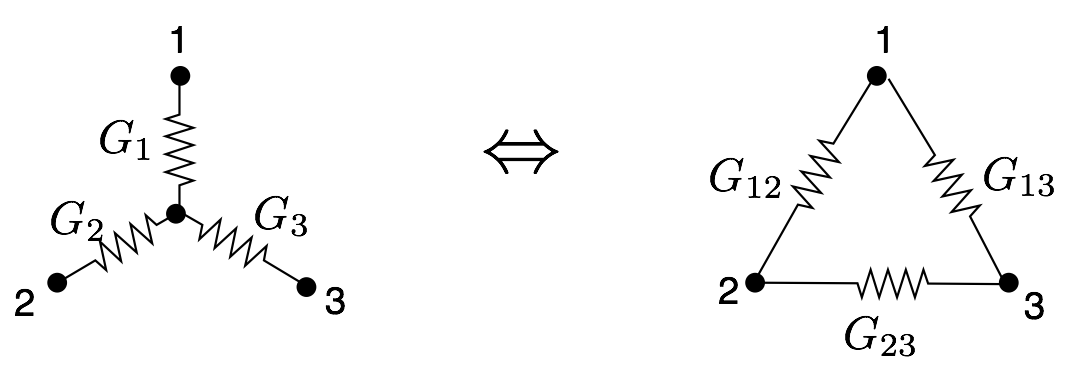
\includegraphics[width=0.6\linewidth]{figs/e2t_3}
\end{center}
La condition d'équivalence est que les deux circuits aient la même matrice de conductances vue de deux accès (par exemple, $1-3$ et $2-3$)

La matrice de conductances aux accès du triangle ${\bf G}_T$ est la matrice de conductances aux n{\oe}uds du circuit avec $3$ comme
n{\oe}ud de référence :
\begin{center}
\begin{minipage}[c]{0.33 \textwidth}
	\begin{center}
	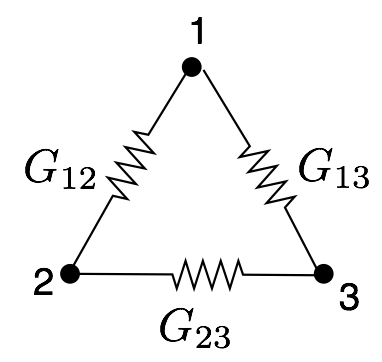
\includegraphics[width=0.7\linewidth]{figs/e2t_2}
	\end{center}
\end{minipage}
\begin{minipage}[c]{0.66 \textwidth}
    par la règle d'inspection, 
	\[{\bf G}_T=
	\left[
	\begin{array}{cc}
	G_{12}+G_{13} & -G_{12}\\
	-G_{12} & G_{12}+G_{23}
	\end{array} \right]\]
\end{minipage}
\end{center}

Construisons maintenant la matrice de conductances aux n{\oe}uds du triangle ${\bf G}_{NE}$ avec $3$ comme n{\oe}ud de référence.
\begin{center}
	\begin{minipage}[c]{0.33 \textwidth}
		\begin{center}
			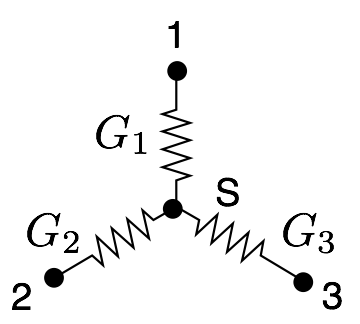
\includegraphics[width=0.7\linewidth]{figs/e2t_1}
		\end{center}
	\end{minipage}
	\begin{minipage}[c]{0.66 \textwidth}
    Par la règle d'inspection, 
	\[{\bf G}_{NE}=
	\begin{array}{c}
	\mathcolor{gray}{1} \\\mathcolor{gray}{2} \\\mathcolor{gray}{S}
	\end{array}
	\left[
	\begin{array}{cc|c}
	G_1 & 0 & -G_1\\
	0 & G_2 & -G_2\\ \hline
	-G_1 & -G_2 & G_1+G_2+G_3
	\end{array} \right]\]
    où le partitionnement en $\mathbf{G}_{aa}$, $\mathbf{G}_{ab}$, $\mathbf{G}_{ba}$ et $\mathbf{G}_{bb}$ est indiqué.
	\end{minipage}
\end{center}
	
Éliminons l'accès $S-3$ en réduisant ${\bf G}_{NE}$ aux 2 accès
``intéressants'' : 
\begin{eqnarray*}
	{\bf G}_E &=&
	\left[
	\begin{array}{cc}
		G_1 & 0\\ 0 & G_2
	\end{array} \right] - \left[
	\begin{array}{c}
		-G_1 \\-G_2
	\end{array}\right] \frac{1}{G_1+G_2+G_3} \left[
	\begin{array}{cc}
		-G_1 & -G_2
	\end{array}\right] \\[6mm] & = & \left[ 
	\begin{array}{cc}\displaystyle 
		\frac{G_1G_2+G_1G_3}{G_1+G_2+G_3} & \displaystyle 
		-\frac{G_1G_2}{G_1+G_2+G_3}\\\displaystyle 
		-\frac{G_1G_2}{G_1+G_2+G_3} & \displaystyle \frac{G_1G_2+G_2G_3}{G_1+G_2+G_3} 
	\end{array}\right]
\end{eqnarray*}

\begin{columns}
  \begin{column}{0.45\textwidth}
    Par identification, on a  pour la transformation étoile $\rightarrow$ triangle :
    \[\begin{array}{c}
    G_{12}=\frac{G_1G_2}{G_1+G_2+G_3}\\[4mm]
    G_{13}=\frac{G_1G_3}{G_1+G_2+G_3}\\[4mm]
    G_{23}=\frac{G_2G_3}{G_1+G_2+G_3}
    \end{array}\]
  \end{column}
  \begin{column}{0.45\textwidth}
    ou en utilisant les résistances des branches : 
    \[\begin{array}{c}
    R_{12}=\frac{R_1R_2+R_2R_3+R_1R_3}{R_3}\\[4mm]
    R_{13}=\frac{R_1R_2+R_2R_3+R_1R_3}{R_2}\\[4mm]
    R_{23}=\frac{R_1R_2+R_2R_3+R_1R_3}{R_1}
    \end{array} \]
  \end{column}
\end{columns}
\vspace{\baselineskip}
On peut de la même manière établir les conditions pour la transformation inverse.

    
\end{frame}

